% What is MIxT used for? And how would users do it in VR?
% How the MIxT application is implemented in GeneNet VR and what it does.
% What are typical network characteristics for this (type of) application? Size, clusters, edges, connectivity, etc?

The Matched Interaction Across Tissues (MIxT) is a system developed by UiT and Concordia University for exploring and comparing transcriptional profiles from two or more matched tissues across individuals \cite{fjukstad_dumeaux_olsen_lund_hallett_bongo_2017}. This system is implemented as a web application and it has a 2-dimensional visualization tool to explore biological networks \footnote{https://mixt-tumor-stroma.bci.mcgill.ca/network}. This tool has, however, some known scalability and visualization problems.

We have used MIxT in GeneNet VR as a case study. In addition, we used this case study in the evaluation since it is a realistic application where we used complex networks that originally didn't scale in the existing web application. In this chapter, we will describe what MIxT is used for, its disadvantages for scaling large biological networks, and the challenges of building a VR visualization system that can solve the visualization and scalability problems.

\section{What is MIxT used for?}
MIxT is a web application for interactive data exploration in system biology developed by UiT and Concordia University. The research was carried out for the study of interactions between the tumor and the blood systemic response of breast cancer patients. In the study, they profiled RNA in blood and matched tumor from 173 patients with breast cancer. The goal of the study was to identify genes and pathways in the primary tumor that are tightly linked to genes and pathways in the patient's systemic response (SR). The SR is the body's response to an infectious or non-infectious insult. A biological pathway is a series of actions among the molecules in a cell that leads to a certain product or change in the cell. The result of the study suggests new ways to monitor breast cancer by looking outside the tumor and studying the patient's systemic response.

MIxT provides an interactive view of networks. In Figure \ref{fig:mixt_webapp}, we show a screenshot from the network view. This view is two-dimensional and the user can do some interactions to explore data, but these are very limited. The users can zoom in and zoom out and also drag and drop with the mouse in the view in order to "move around". Also, by hovering on a node, the user can see the name of that node. By clicking on a node, the user goes to another page with more detailed biological information about that gene.

\begin{figure}[h!]
    \setlength{\tempheight}{15ex}
    \centering
    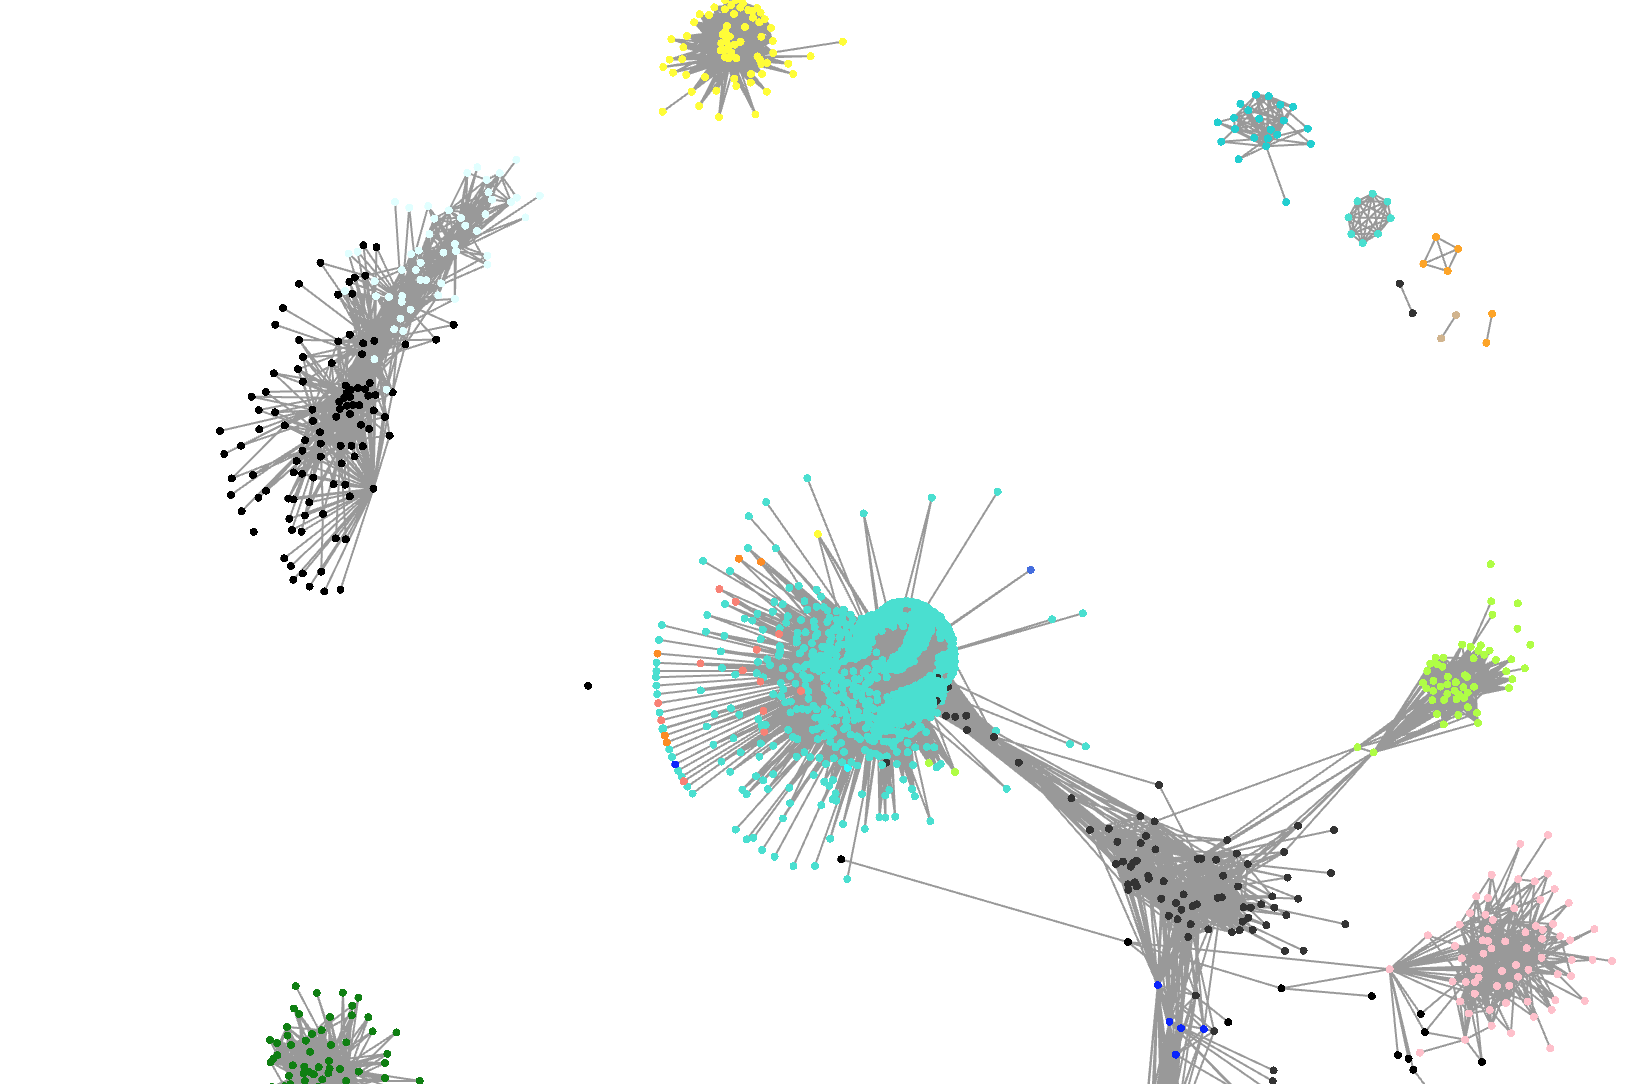
\includegraphics[width=\textwidth]{mixt_webapp}
    \caption{Screenshot from the network view in the MIxT web application.}
    \label{fig:mixt_webapp}
\end{figure}

An evident problem in this view appears when we start to explore the network. The clusters have many nodes and each node can have multiple edges, so the graph ends up looking like a hairball and it is not easy to explore (see Figure \ref{fig:mixt_hairball} for a screenshot of this problem from MIxT). In addition, the edges need to be rendered every time the user interacts with the network. It may take a few seconds until the user can view all the edges that are in the view frame. This is a problem since the user needs to do many interactions when exploring the network. The visualization process becomes cumbersome and tedious in MIxT.

\begin{figure}[h!]
    \setlength{\tempheight}{15ex}
    \centering
    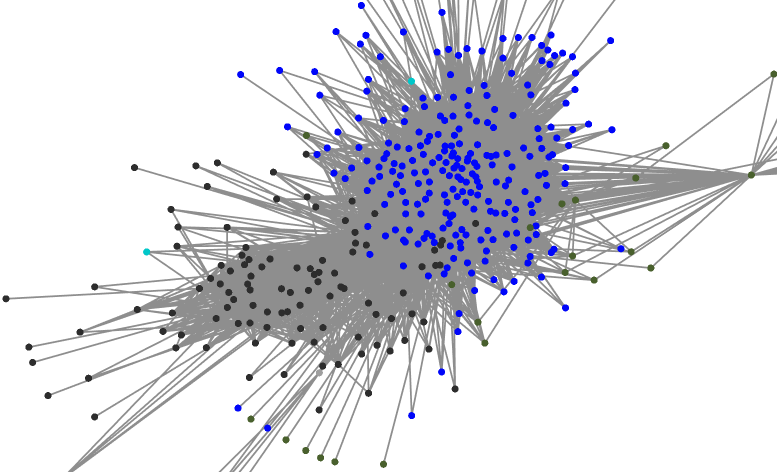
\includegraphics[width=\textwidth]{mixt_hairball}
    \caption{Hairball problem in the network view in MIxT.}
    \label{fig:mixt_hairball}
\end{figure}

\section{MIxT in VR}
We have implemented a Virtual Reality version of the network view from MIxT in order to solve some scalability and visualization problems. In addition to the original challenges that the network visualizer has, there are other challenges that we have to take into account in VR. In this section, we are going to explain these challenges and how we solved them in GeneNet VR.

When moving the original visualization system to VR, we have a new dimension in addition to immersion. Having a new dimension is an advantage when we want to visualize high-dimensional data, like biological networks. However, we need to cope with new problems like object occlusion. When the user visualizes the network from a particular angle, the nodes and edges that are in front of the user's viewpoint may hide other nodes and edges that are behind these. To solve this problem, we need to give the user the possibility to view the network from different angles. In GeneNet VR we have implemented a locomotion solution that allows the user to teleport to other parts of the scene. The user can also rotate the viewpoint to the right or to the left. In addition, the user can also move the network around by using the VR controller.

As we mentioned before, the original network view from MIxT has some visualization problems. The network looks like a hairball and it's hard to explore it. In GeneNet VR we solve this problem by showing only the edges from the nodes that the user wants to explore. This solution reduces the amount of information that is shown, but it higher interactivity, so that the user can easily visualize the information. In GeneNet VR, we have implemented a node selector that allows the user to select a particular node using a laser pointer. When the laser collides with a node, the edges of this node are shown. Also, the user can scale up and down the network by using the VR controllers. In addition, a filtering menu was implemented in GeneNet VR, where the user can filter out the information from the network that is not relevant.

We have added the possibility to compare two datasets in real-time in GeneNet VR. This can be very useful for bioinformaticians when they work with several datasets like in MIxT. To compare two networks, the user can use a UI slider to visualize two datasets at the same time, creating what we call a morphing effect. To help the user distinguish from one dataset to another, we use linear interpolation for both the color of the nodes and their position.

\section{Network characteristics}
The networks from MIxT that we use in our case study are also known as gene co-expression networks (GCN) in biology. They are undirected graphs; meaning that the nodes can be connected together with bidirectional edges. In a GCN, the nodes represent genes and an edge between two nodes represents a significant co-expression relationship. As we previously showed in Figure \ref{fig:mixt_webapp}, the nodes are in the networks are also organized in clusters and colors. Each cluster corresponds to a module, which is a subgraph where the genes are highly connected and where these genes are part of a common biological process that causes many interactions among themselves.
